\subsection{Berechnung}
Um einen Ball durch die Schwingräder mit einem gewissen Anpressdruck zu führen, wird ein Drehmoment benötigt. Dazu betrachten wir den Tennisball als eine Feder mit der Federkonstante k.
Zur Ermittlung der Federkonstante k wurde der Ball mit einer Masse m beschwert, und die Verschiebung x gemessen.

\begin{figure}[h!]
	\centering
	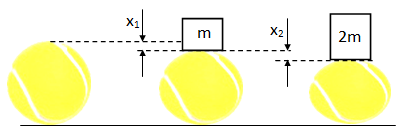
\includegraphics[width=0.4\textwidth]{Enddokumentation/Anhang/Bilder/KompressionBaelle.png}
	\caption{Prinzip der k-Bestimmung}
	\label{fig:BallKomp}
\end{figure}

\begin{table}[h!]
	\begin{tabular}{p{1.5cm}p{2cm}}
		Gewicht & Auslenkung\\
		\hline
		1kg & 1 mm\\
		2kg & 2 mm\\
		3kg & 3 mm\\
	\end{tabular}
	\centering
	\caption{Prinzip der k-Bestimmung}
	\label{tab:BallKompErgebnis}
\end{table}
Da $x_1$ und $x_2$ in etwa gleich gross sind, kann von einer linearen Federkonstante ausgegangen werden. Damit kann die Kraft, die durch das Stauchen des Balles entsteht mit der Formel
\begin{equation}  
 F_s=2\cdot k \cdot \Delta x 
 \end{equation}
bestimmt werden. Die Federkonstante k beträgt $9.8\frac{N}{mm}$ Das entstehende Drehmoment, wird mit trigonometrischer Beziehung hergeleitet. 

\begin{equation}  
 	M = R_S \cdot F_t
 \end{equation}
\begin{equation}  
	F_t = F_s \cdot \sin(\alpha)
\end{equation}
\begin{equation}  
	F_s = 2\cdot k \cdot \Delta x 
\end{equation}
\begin{figure}[h!]
	\centering
	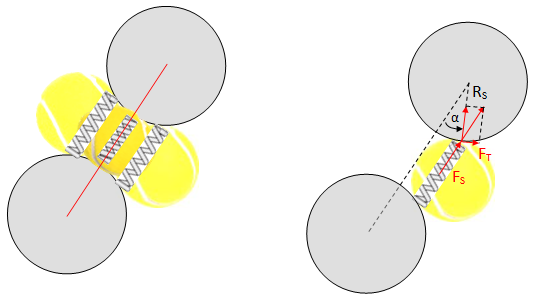
\includegraphics[width=0.4\textwidth]{Enddokumentation/Anhang/Bilder/PrinzipKompression.png}
	\caption{Prinzip der Kompression}
	\label{fig:PrinzipBallKomp}
\end{figure}
Da $\Delta x$ vom Winkel $\alpha$ abhängt, muss die folgende Abhängigkeit gelten:

\begin{equation}  
	\alpha = R_s \cdot \frac{1}{\cos(\alpha)} \\ b = a - R_s = R_s \left( \frac{1}{\cos(\alpha)}-1\right)   
\end{equation}